\documentclass[usenatbib,twocolumn]{mnras}
\usepackage{cuted}
%\linespread{2.0}
\usepackage[utf8]{inputenc}
\usepackage[T1]{fontenc}
\usepackage{graphicx}
\usepackage{longtable}
\usepackage{wrapfig}
\usepackage{rotating}
\usepackage[normalem]{ulem}
\usepackage{amsmath}
\usepackage{amssymb}
\usepackage{capt-of}
\usepackage{hyperref}
\usepackage{tensor}
\usepackage{amsmath}
\usepackage{caption}
\usepackage{tabularx}
\usepackage{subcaption}
\usepackage{pdfpages}
\usepackage{float}
\usepackage{booktabs}
\usepackage{enumitem}
\usepackage{graphicx}
\usepackage{tensor}
\usepackage{wasysym}
\usepackage{mathtools}
\usepackage{xcolor}
\usepackage{cancel}
\DeclarePairedDelimiter{\abs}{|}{|}
\DeclarePairedDelimiter{\norm}{||}{||}
\DeclarePairedDelimiter{\p}{(}{)}
\DeclarePairedDelimiter{\we}{\langle}{\rangle}

\title[Apsidal Precession in MMR]{Architecture Sculpting by Apsidal Precession in Mean Motion Resonances}
\author[Laune et al.]{ JT Laune,$^{1}$ Laetitia Rodet,$^{1}$ and Dong
  Lai$^{1}$
  \\
  $^{1}$Department of Astronomy, Cornell Center for Astrophysics and
  Planetary Science, Cornell University, Ithaca, NY 14853, USA \\}

\begin{document}
\maketitle

\section{Introduction}
    Planets have long been expected to migrate in their natal protoplanetary disks \citep[PPDs; e.g.][]{nelson00_migrat_growt_protop_protos_discs}.

    An orbiter in a potential with a nonzero quadrupole moment will undergo apsidal precession. 
    Common astrophysical scenarios with a nonzero quadrupole include a planet being perturbed secularly by a disk or another planet as well as a planet orbiting an oblate star (with a $J_2$ moment). 
    In the case of a disk, a planet's longitude of perihelion $\varpi$ will precess at a rate
    \begin{equation}
        \frac{\dot\varpi}{n} \simeq 0.0004\left(\frac{a}{1~\rm{au}}\right)^3\left(\frac{M_d/M}{0.1}\right)\left(\frac{3~\rm{au}}{r_{\rm in}}\right)^2\left(\frac{10~\rm{au}}{r_{\rm out}}\right)
%= \frac34 \frac{n}{M}\int_{r_{\rm in}}^{r_{\rm out}} \Sigma(r_d)\left(\frac{a}{r_d}\right)^3 dm_d
    \end{equation}
    for a star of mass $M$, a disk of mass $M_d$ extending from $r_{\rm in}$ to $r_{\rm out}$ ($\gg r_{\rm in}$), and planet at semimajor axis (SMA) $a$ and mean motion $n$.


\section{Coplanar Eccentric Restricted 3-Body Problem}
\label{sec:CER3BP}
The \emph{Coplanar Eccentric Restricted 3-Body Problem} (CER3BP) is the problem of a test particle orbiting a primary of mass $M$ near a $p:q$ MMR for a coplanar ($i=0^\circ$) perturber of mass $m_p$.
We restrict our attention to an interior first order resonance, $j:j+1$.

\subsection{Hamiltonian and Equations of Motion}
The non-dissipative problem for a $j:j+1$ resonance is a non-autonomous dimensionless Hamiltonian with two degrees of freedom,
\begin{align}
    \sqrt{a} &\longleftrightarrow \lambda,\\
    \sqrt{a}(1-\sqrt{1-e^2})\simeq \frac12\sqrt{a}e^2&\longleftrightarrow -\varpi.
\end{align}
The Hamiltonian of the system is 
\begin{align}
    \label{eq:TPH}
    \mathcal H=&-\frac{GM}{2a}
    +\frac{GMm_p}{a_p}\left\{
        f_1e\cos((j+1)n_p(a_p)t-j\lambda-\varpi)\right.\\
        &\left. +f_2e_p\cos((j+1)n_p(a_p)t-j\lambda-\varpi_p)
    \right\}.\nonumber
\end{align}
The resonant arguments are 
\begin{align}
    \theta=(j+1)\tau -j\lambda-\varpi,\\
    \theta_p=(j+1)\tau -j\lambda-\varpi_p,
\end{align}
where $\tau=n_p t$ is the dimensionless time. For a nominal choice of $a_p=1~\rm{au}$, $n_p = 2\pi~\mathrm{rad}/\mathrm{yr}$.

\subsection{Dissipation}
We add dissipation to the system as
\begin{align}
 \frac{d}{d\tau} a&=- \frac{a}{(2\pi T_{m})} - \frac{2 a e^{2}}{(2\pi T_{e})},\\
 \frac{d}{d\tau} e&=- \frac{e}{(2\pi T_{e})},\\
\end{align}
where $T_e$ and $T_m$ are the test particle's eccentricity- and SMA-damping timescales, respectively. Since the test particle is inside the orbit of $m_p$, we set $T_m<0$ and let the test particle migrate outwards.


\subsection{Constant Apsidal Precession}
\label{sec:}
We add the term $-\pi\Gamma\simeq = -\pi\left(\frac12\sqrt{\alpha}e^2\right)$ to the Hamiltonian \ref{eq:TPH}, which induces the precession term
\begin{equation}
    \left(\frac{d\varpi}{d\tau}\right)_{\rm ext} = \pi.
\end{equation}

\subsection{Reducing the Hamiltonian}
Through a series of canonical transformations and approximations, the Hamiltonian \ref{eq:TPH} (including the apsidal precession terms) can be reduced to 
\begin{align}
    \mathcal H(M,R) \simeq& - \frac{3 M^{2} j^{\frac{2}{3}} \left(j + 1\right)^{\frac{4}{3}}}{2} + \frac{M \pi_{2}}{\mu^{\frac{2}{3}}} 
    - \frac{R \left( \pi_{1} - \pi_{2}\right)}{\mu^{\frac{2}{3}}}
    \nonumber\\
    &+ \sqrt{2} \sqrt{R} \left(f_{1} \cos{\left(m + r \right)}
        +\frac{e_{p} f_{2} \left(\pi_{1} - \pi_{2}\right) \cos{\left(r \right)}}{f_{1} \mu}\right)
\end{align}
where the new canonical momentum-coordinate pairs are
\begin{align}
    R =& \frac{\sqrt{\alpha} e^{2} f_{1}^{2} - 2 \sqrt[4]{\alpha} e e_{p} f_{1} f_{2} \cos{\left(\pi_{2} \tau - \varpi \right)} + e_{p}^{2} f_{2}^{2}}{2 f_{1}^{2} \mu^{\frac{2}{3}}}\\
    &\leftrightarrow r = \mathrm{atan}\frac{e \sin{\left(g_{1} \right)}}{ \frac{e_{p} f_{2}}{f_{1} \sqrt[4]{a}}- e \cos{\left(g_{1} \right)}},\\
    M=&\frac{\sqrt{\alpha}- (j/(j+1))^{1/3} }{j \mu^{\frac{2}{3}}}
    \leftrightarrow m =  j l - \tau \left(j + 1\right),
\end{align}
and the momenta are now $M\sim R \sim\mathcal O(1)$.


\section{Coplanar Comparable Mass Problem}
The \emph{Coplanar Comparable Mass Problem} (CCMP) is the problem of two coplanar comparable mass (mass ratio $q=m_1/m_2\sim\mathcal O(1)$) near a $p:q$ MMR.

\subsection{Hamiltonian and Equations of Motion}
The non-dissipative problem for a $j:j+1$ resonance is an autonomous dimensionless Hamiltonian with 4 degrees of freedom,
\begin{align}
    \sqrt{a_1}&\leftrightarrow \lambda_1,\\
    \sqrt{a_1}(1-\sqrt{1-e_1^2})\simeq\frac12\sqrt{a_1}e_1^2&\leftrightarrow -\varpi_1,\\
    \sqrt{a_2}&\leftrightarrow \lambda_2,\\
    \sqrt{a_2}(1-\sqrt{1-e_2^2})\simeq\frac12\sqrt{a_2}e_2^2&\leftrightarrow -\varpi_2,
\end{align}
The Hamiltonian of the system is
\begin{align}
    \label{eq:CCMP_H}
    \mathcal H=
    &- \frac{G M m_{2}}{2 a_{2}} - \frac{G M m_{2} q}{2 a_{1}} \\
    &- \frac{G m_{2}^{2} q}{a_{2}} \left(e_{1} f_{1} \cos{\theta_1} + e_{2} f_{2} \cos{\theta_2}\right) \\
    &- \frac{G m_{2}^{2} q \left(e_{1} e_{2} f_{4} \cos{\left(g_{1} - g_{2} \right)} + f_{3} \left(e_{1}^{2} + e_{2}^{2}\right)\right)}{a_{2}},
\end{align}
where the two resonant arguments are
\begin{align}
    \theta_1 &=\lambda_{2} \left(j + 1\right) - j \lambda_{1}-\varpi_{1}, \\
    \theta_2 &= \lambda_{2} \left(j + 1\right)- j \lambda_{1}-\varpi_{2}.
\end{align}
We now switch to dimensionless units by scaling the masses by $M$,
\begin{align}
    m_1 = \mu_1 M,\\
    m_2 = \mu_2 M,
\end{align}
the SMAs by $a_0$,
\begin{align}
    a_1 &= \bar a_1a_0,\\
    a_2 &= \bar a_2a_0,
\end{align}
the time by $n_0^{-1} = \sqrt{a_0^{3}/GM}$,
\begin{align}
    t &= \tau/n_0,
\end{align}
and the Hamiltonian by,
\begin{align}
    \mathcal H = \bar{\mathcal{H}} \left(\frac{GMm_2(1+q)}{a_2}\right).
\end{align}
The angular angular momenta are therefore in the units
\begin{align}
    \Lambda_1 = \bar\Lambda_1 \mu_2(1+q)\sqrt{GMa_{0}}.
\end{align}
From here on out all coordinates and momenta will be assumed to be dimensionless and we will drop the bars.
We will use nominal values of $a_0=1~\mathrm{au}$ and $M=1~M_\odot$ so that time is in years and $\tau=2\pi t$.
We then derive the equations of motion of the system from Hamilton's equations. For a list of the full equations, see Appendix~\ref{sec:eqCCMP}.

\subsection{Dissipation}\label{sec:cm-dis}
We add dissipation to the system as
\begin{align}
 \frac{d}{d\tau} a_1&=- \frac{a_{1}}{(2\pi T_{m,1})} - \frac{2 a_{1} e_{1}^{2}}{(2\pi T_{e,1})},\\
 \frac{d}{d\tau} a_2&=- \frac{a_{2}}{(2\pi T_{m,2})} - \frac{2 a_{2} e_{2}^{2}}{(2\pi T_{e,2})},\\
 \frac{d}{d\tau} e_1&=- \frac{e_{1}}{(2\pi T_{e,1})},\\
 \frac{d}{d\tau} e_2&=- \frac{e_{2}}{(2\pi T_{e,2})}.
\end{align}
For $q<1$, we choose $T_{m,2}=2\times10^7$, $T_{m,1}=\infty$, $T_{e,1}=1\times10^5$, and $T_{e,2}=qT_{e,1}$.
For $q>1$, we choose $T_{m,1}=-2\times10^7$, $T_{m,2}=\infty$, $T_{e,2}=1\times10^5$, and $T_{e,1}=T_{e,1}/q$.
This is equivalent to a disk aspect ratio of $h\sim 0.027$.

A typical capture scenario for is demonstrated in Figure~\ref{fig:cm-control}.

\begin{figure}
    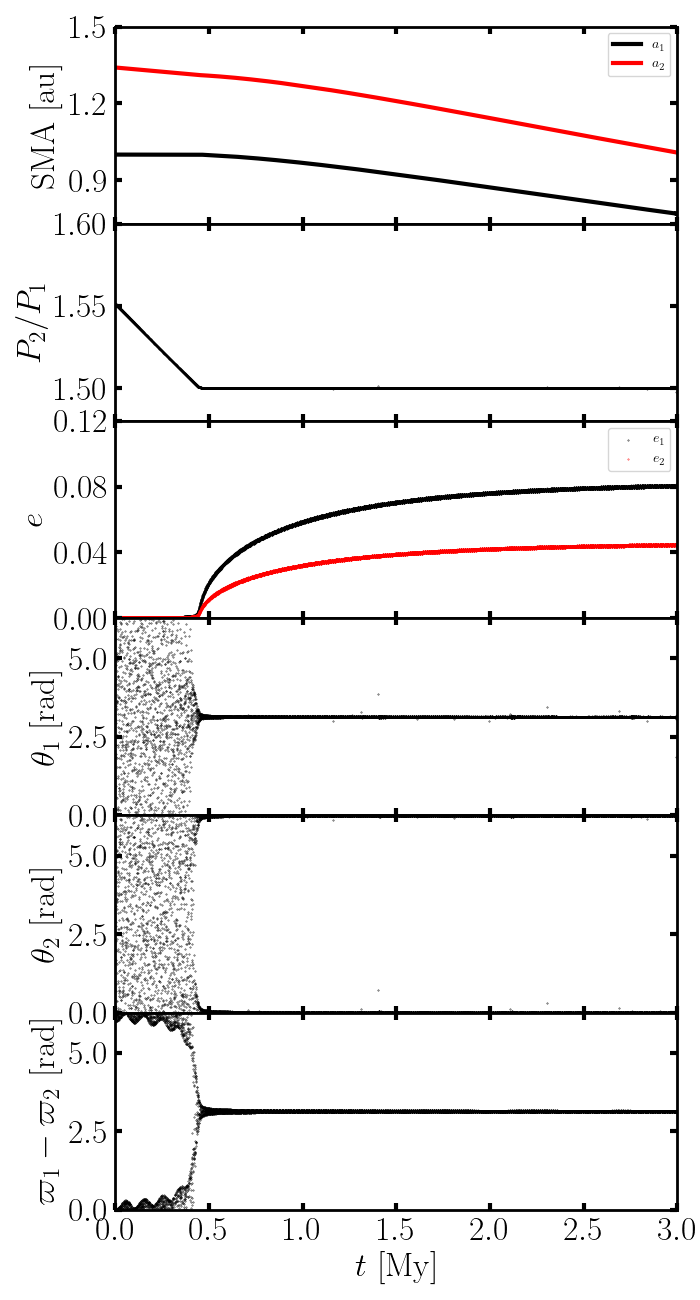
\includegraphics[width=0.4\textwidth]{cm_0_0.png}
\caption{Mean motion resonance capture for $m_1=1~M_\oplus$ and $m_2=2~M_\oplus$. The dissipative timescales are given in Section \ref{sec:cm-dis}. The two planets are initiated just wide of resonance at a period ratio of $P_2/P_1=1.55$. After around 0.5~Myr, the planets cross the 2:3 MMR and are captured, indicated by the tight libration of $\theta_1$ and $\theta_2$. The periapses transition from being aligned ($\Delta\varpi=\varpi_1-\varpi_2=0^\circ$) to anti-aligned ($\Delta\varpi=\varpi_1-\varpi_2=180^\circ$).}
    \label{fig:cm-control}
\end{figure}

\begin{figure}
    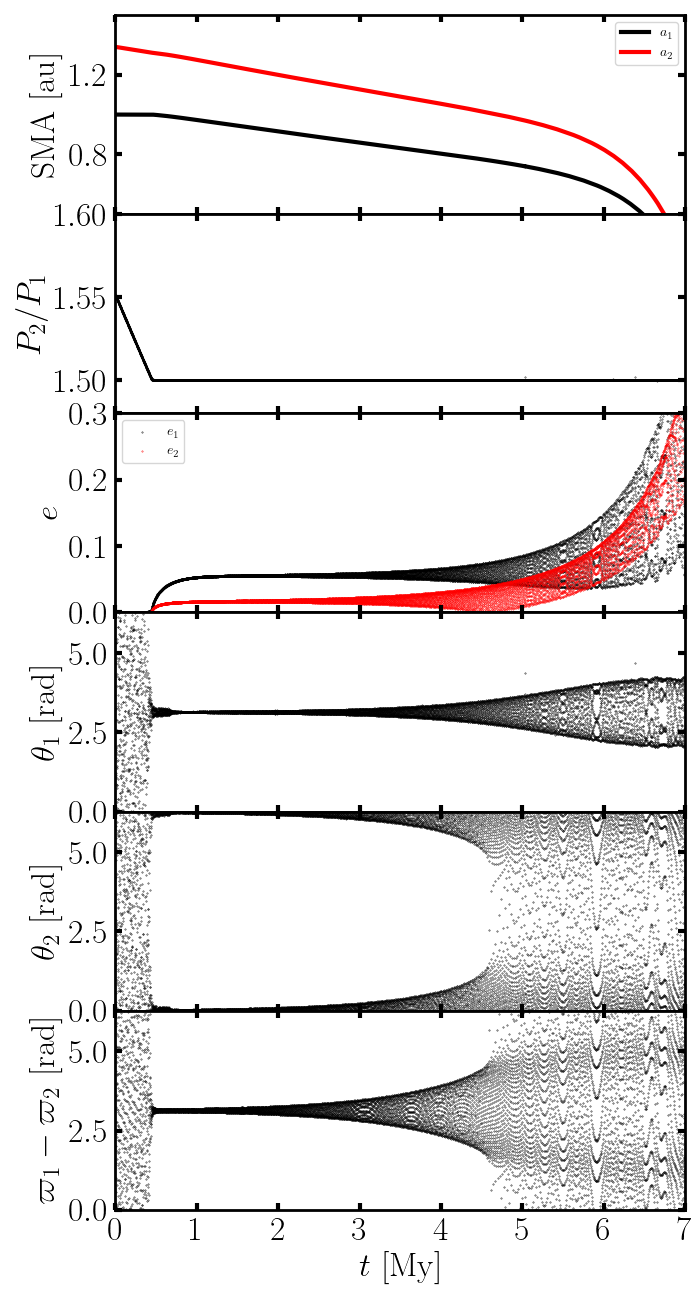
\includegraphics[width=0.4\textwidth]{cm_1e-4_2e-4.png}
    \caption{The same as Figure~\ref{fig:cm-control} but with $\pi_1=10^{-4}$ and $\pi_2=2\times10^{-4}$ ($\Delta\dot\varpi=\pi_1-\pi_2=-10^{-4}>0$). After around 4.5~Myr, $\theta_2$ begins circulating and eccentricities increase to orbit-crossing values (resulting in instability).}
    \label{fig:cm-neg-dDpom}
\end{figure}

\begin{figure}
    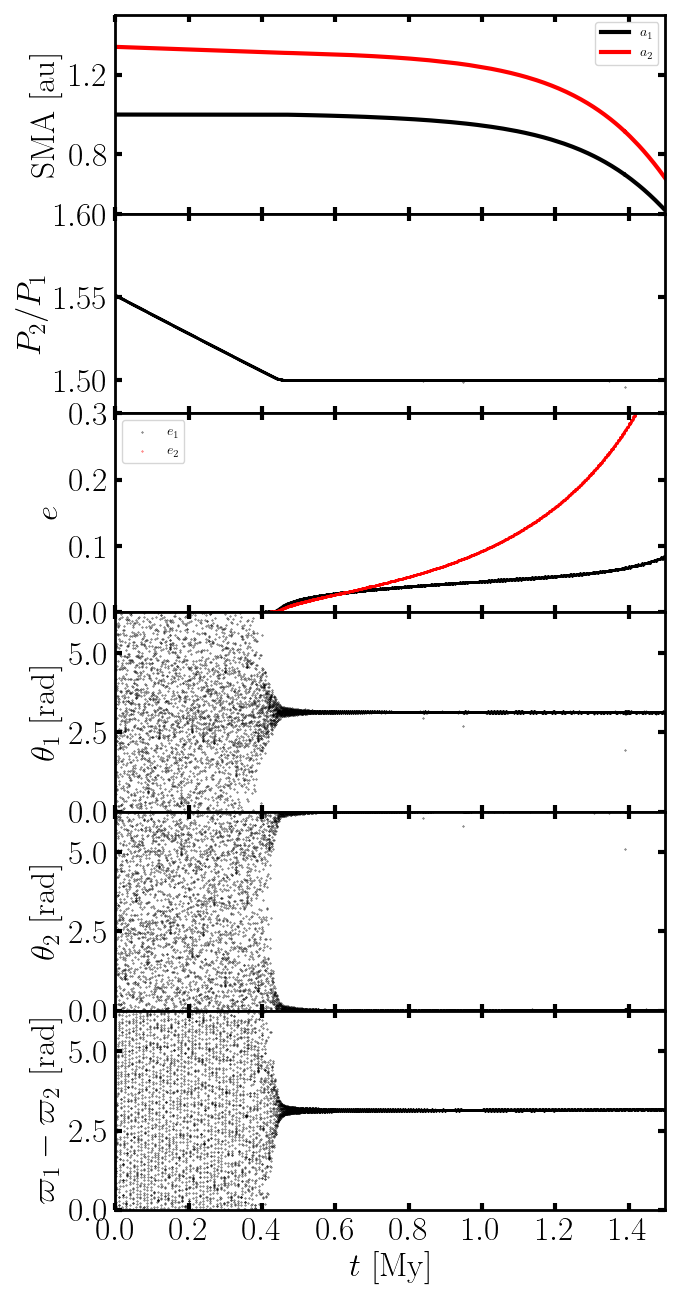
\includegraphics[width=0.4\textwidth]{cm_2e-4_1e-4.png}
    \caption{The same as Figure~\ref{fig:cm-control} but with $\pi_1=2\times10^{-4}$ and $\pi_2=10^{-4}$ ($\Delta\dot\varpi=\pi_1-\pi_2=10^{-4}>0$). After capture, $\theta_1$ and $\theta_2$ continue to librate but $e_2$ increases to orbit-crossing values (resulting in instability).
    }
    \label{fig:cm-pos-dDpom}
\end{figure}

\subsection{Constant Apsidal Precession}
We add the terms $-\Gamma_1\pi_1-\Gamma_2\pi_2$ to the Hamiltonian (\ref{eq:CCMP_H}) to induce apsidal precession at the constant angular frequencies $\pi_1,\pi_2$ on $\varpi_1,\varpi_2$, respectively. In particular, the following terms are added to the equations of motion,
\begin{align}
    \left(\frac{d\varpi_1 }{d\tau}\right)_{\rm ext} = \pi_1, \\
    \left(\frac{d\varpi_2 }{d\tau}\right)_{\rm ext} = \pi_2.
\end{align}

\subsubsection{$\pi_1-\pi_2<0$}
See Figure~\ref{fig:cm-neg-dDpom}.

\subsubsection{$\pi_1-\pi_2>0$}
See Figure~\ref{fig:cm-pos-dDpom}.








\clearpage
\bibliography{bibliography}
\bibliographystyle{mnras}
\clearpage
\onecolumn
\appendix
\section{Equations solved in the CER3BP}
We take the total energy of the particle as the Hamiltonian, as in Section \ref{sec:CER3BP} (equation \ref{eq:TPH}), and adopt the notation therein.
Utilizing a type 2 time-dependent generating function, $F=- \Theta_{0} \left(- j \lambda + \tau \left(j + 1\right)\right)$, we transform to the variables
\begin{equation}
    \Theta_{0} = \frac{\Lambda}{j} \longleftrightarrow
    \theta_0 = j \lambda - \tau \left(j + 1\right).
\end{equation}

The new Hamiltonian is
\begin{equation}
    \mathcal H_0 = - \Theta_{0} j - \Theta_{0} + e_{p} f_{2} \mu \cos{\left(\theta_{0} \right)} + \sqrt{2} f_{1} \mu \sqrt{\frac{\sqrt{X^{2} + Y^{2}}}{\Theta_{0} j}} \cos{\left(\theta_{0} - \operatorname{atan}_{2}{\left(Y,X \right)} \right)} - \frac{1}{2 \Theta_{0}^{2} j^{2}},
\end{equation}
and, by Hamilton's equations,
\begin{align}
   \dot\theta_0 &= - j - 1 - \frac{\sqrt{2} f_{1} \mu \sqrt{\frac{\sqrt{X^{2} + Y^{2}}}{\Theta_{0} j}} \cos{\left(\theta_{0} - \operatorname{atan}_{2}{\left(Y,X \right)} \right)}}{2 \Theta_{0}} + \frac{1}{\Theta_{0}^{3} j^{2}}\\
   \dot\Theta_0 &= \mu \left(e_{p} f_{2} \sin{\left(\theta_{0} \right)} + \sqrt{2} f_{1} \sqrt{\frac{\sqrt{X^{2} + Y^{2}}}{\Theta_{0} j}} \sin{\left(\theta_{0} - \operatorname{atan}_{2}{\left(Y,X \right)} \right)}\right)\\
   \dot X &= \frac{\sqrt{2} f_{1} \mu \sqrt{\frac{\sqrt{X^{2} + Y^{2}}}{\Theta_{0} j}} \left(2 X \sin{\left(\theta_{0} - \operatorname{atan}_{2}{\left(Y,X \right)} \right)} + Y \cos{\left(\theta_{0} - \operatorname{atan}_{2}{\left(Y,X \right)} \right)}\right)}{2 \left(X^{2} + Y^{2}\right)} \\
   \dot Y &= \frac{\sqrt{2} f_{1} \mu \sqrt{\frac{\sqrt{X^{2} + Y^{2}}}{\Theta_{0} j}} \left(- X \cos{\left(\theta_{0} - \operatorname{atan}_{2}{\left(Y,X \right)} \right)} + 2 Y \sin{\left(\theta_{0} - \operatorname{atan}_{2}{\left(Y,X \right)} \right)}\right)}{2 \left(X^{2} + Y^{2}\right)}
\end{align}
\section{Equations solved in the CCMP}\label{sec:eqCCMP}
From Hamilton's equations and the CCMP Hamiltonian~\ref{eq:CCMP_H}, the equations of motion for the system are
\begin{align}
    \frac{d}{d\tau} \lambda_1 =& \frac{q}{a_{1}^{\frac{3}{2}}} + \frac{1}{a_{1}^{\frac{3}{2}}}
    \frac{e_{1}^{2} f_{3} \mu_{2} q}{\sqrt{a_{1}} a_{2}} + \frac{e_{1}^{2} f_{3} \mu_{2}}{\sqrt{a_{1}} a_{2}} + \frac{e_{1} e_{2} f_{4} \mu_{2} q \cos{\left(\theta_{1} - \theta_{2} \right)}}{2 \sqrt{a_{1}} a_{2}} + \frac{e_{1} e_{2} f_{4} \mu_{2} \cos{\left(\theta_{1} - \theta_{2} \right)}}{2 \sqrt{a_{1}} a_{2}} + \frac{e_{1} f_{1} \mu_{2} q \cos{\left(\theta_{1} \right)}}{2 \sqrt{a_{1}} a_{2}} + \frac{e_{1} f_{1} \mu_{2} \cos{\left(\theta_{1} \right)}}{2 \sqrt{a_{1}} a_{2}},\\
    \frac{d}{d\tau} \Lambda_1 =&\frac{e_{1} f_{1} j \mu_{2} q \sin{\left(\theta_{1} \right)}}{a_{2}} + \frac{e_{2} f_{2} j \mu_{2} q \sin{\left(\theta_{2} \right)}}{a_{2}}, \\
    \frac{d}{d\tau} \lambda_2 =& \frac{q}{a_{2}^{\frac{3}{2}}} + \frac{1}{a_{2}^{\frac{3}{2}}}
    \frac{2 e_{1}^{2} f_{3} \mu_{2} q^{2}}{a_{2}^{\frac{3}{2}}} + \frac{2 e_{1}^{2} f_{3} \mu_{2} q}{a_{2}^{\frac{3}{2}}} + \frac{5 e_{1} e_{2} f_{4} \mu_{2} q^{2} \cos{\left(\theta_{1} - \theta_{2} \right)}}{2 a_{2}^{\frac{3}{2}}} + \frac{5 e_{1} e_{2} f_{4} \mu_{2} q \cos{\left(\theta_{1} - \theta_{2} \right)}}{2 a_{2}^{\frac{3}{2}}} \nonumber\\
    &+ \frac{2 e_{1} f_{1} \mu_{2} q^{2} \cos{\left(\theta_{1} \right)}}{a_{2}^{\frac{3}{2}}} + \frac{2 e_{1} f_{1} \mu_{2} q \cos{\left(\theta_{1} \right)}}{a_{2}^{\frac{3}{2}}} + \frac{3 e_{2}^{2} f_{3} \mu_{2} q^{2}}{a_{2}^{\frac{3}{2}}} + \frac{3 e_{2}^{2} f_{3} \mu_{2} q}{a_{2}^{\frac{3}{2}}} + \frac{5 e_{2} f_{2} \mu_{2} q^{2} \cos{\left(\theta_{2} \right)}}{2 a_{2}^{\frac{3}{2}}} + \frac{5 e_{2} f_{2} \mu_{2} q \cos{\left(\theta_{2} \right)}}{2 a_{2}^{\frac{3}{2}}},  \\
    \frac{d}{d\tau} \Lambda_2 =&- \frac{e_{1} f_{1} j \mu_{2} q \sin{\left(\theta_{1} \right)}}{a_{2}} - \frac{e_{1} f_{1} \mu_{2} q \sin{\left(\theta_{1} \right)}}{a_{2}} - \frac{e_{2} f_{2} j \mu_{2} q \sin{\left(\theta_{2} \right)}}{a_{2}} - \frac{e_{2} f_{2} \mu_{2} q \sin{\left(\theta_{2} \right)}}{a_{2}}, \\
    \frac{d}{d\tau} \gamma_1 =&- \frac{2 f_{3} \mu_{2} q}{\sqrt{a_{1}} a_{2}} - \frac{2 f_{3} \mu_{2}}{\sqrt{a_{1}} a_{2}} - \frac{e_{2} f_{4} \mu_{2} q \cos{\left(\theta_{1} - \theta_{2} \right)}}{\sqrt{a_{1}} a_{2} e_{1}} - \frac{e_{2} f_{4} \mu_{2} \cos{\left(\theta_{1} - \theta_{2} \right)}}{\sqrt{a_{1}} a_{2} e_{1}} - \frac{f_{1} \mu_{2} q \cos{\left(\theta_{1} \right)}}{\sqrt{a_{1}} a_{2} e_{1}} - \frac{f_{1} \mu_{2} \cos{\left(\theta_{1} \right)}}{\sqrt{a_{1}} a_{2} e_{1}}, \\
    \frac{d}{d\tau} \Gamma_1 =&- \frac{e_{1} e_{2} f_{4} \mu_{2} q \sin{\left(\theta_{1} - \theta_{2} \right)}}{a_{2}} - \frac{e_{1} f_{1} \mu_{2} q \sin{\left(\theta_{1} \right)}}{a_{2}},\\
    \frac{d}{d\tau} \gamma_2 =&- \frac{e_{1} f_{4} \mu_{2} q^{2} \cos{\left(\theta_{1} - \theta_{2} \right)}}{a_{2}^{\frac{3}{2}} e_{2}} - \frac{e_{1} f_{4} \mu_{2} q \cos{\left(\theta_{1} - \theta_{2} \right)}}{a_{2}^{\frac{3}{2}} e_{2}} - \frac{2 f_{3} \mu_{2} q^{2}}{a_{2}^{\frac{3}{2}}} - \frac{2 f_{3} \mu_{2} q}{a_{2}^{\frac{3}{2}}} - \frac{f_{2} \mu_{2} q^{2} \cos{\left(\theta_{2} \right)}}{a_{2}^{\frac{3}{2}} e_{2}} - \frac{f_{2} \mu_{2} q \cos{\left(\theta_{2} \right)}}{a_{2}^{\frac{3}{2}} e_{2}}, \\
    \frac{d}{d\tau} \Gamma_2 =&\frac{e_{1} e_{2} f_{4} \mu_{2} q \sin{\left(\theta_{1} - \theta_{2} \right)}}{a_{2}} - \frac{e_{2} f_{2} \mu_{2} q \sin{\left(\theta_{2} \right)}}{a_{2}} .
\end{align}

\end{document}